\section{Model}

\begin{frame}
	\frametitle{Model}
				\begin{figure}[p]
					\centering
					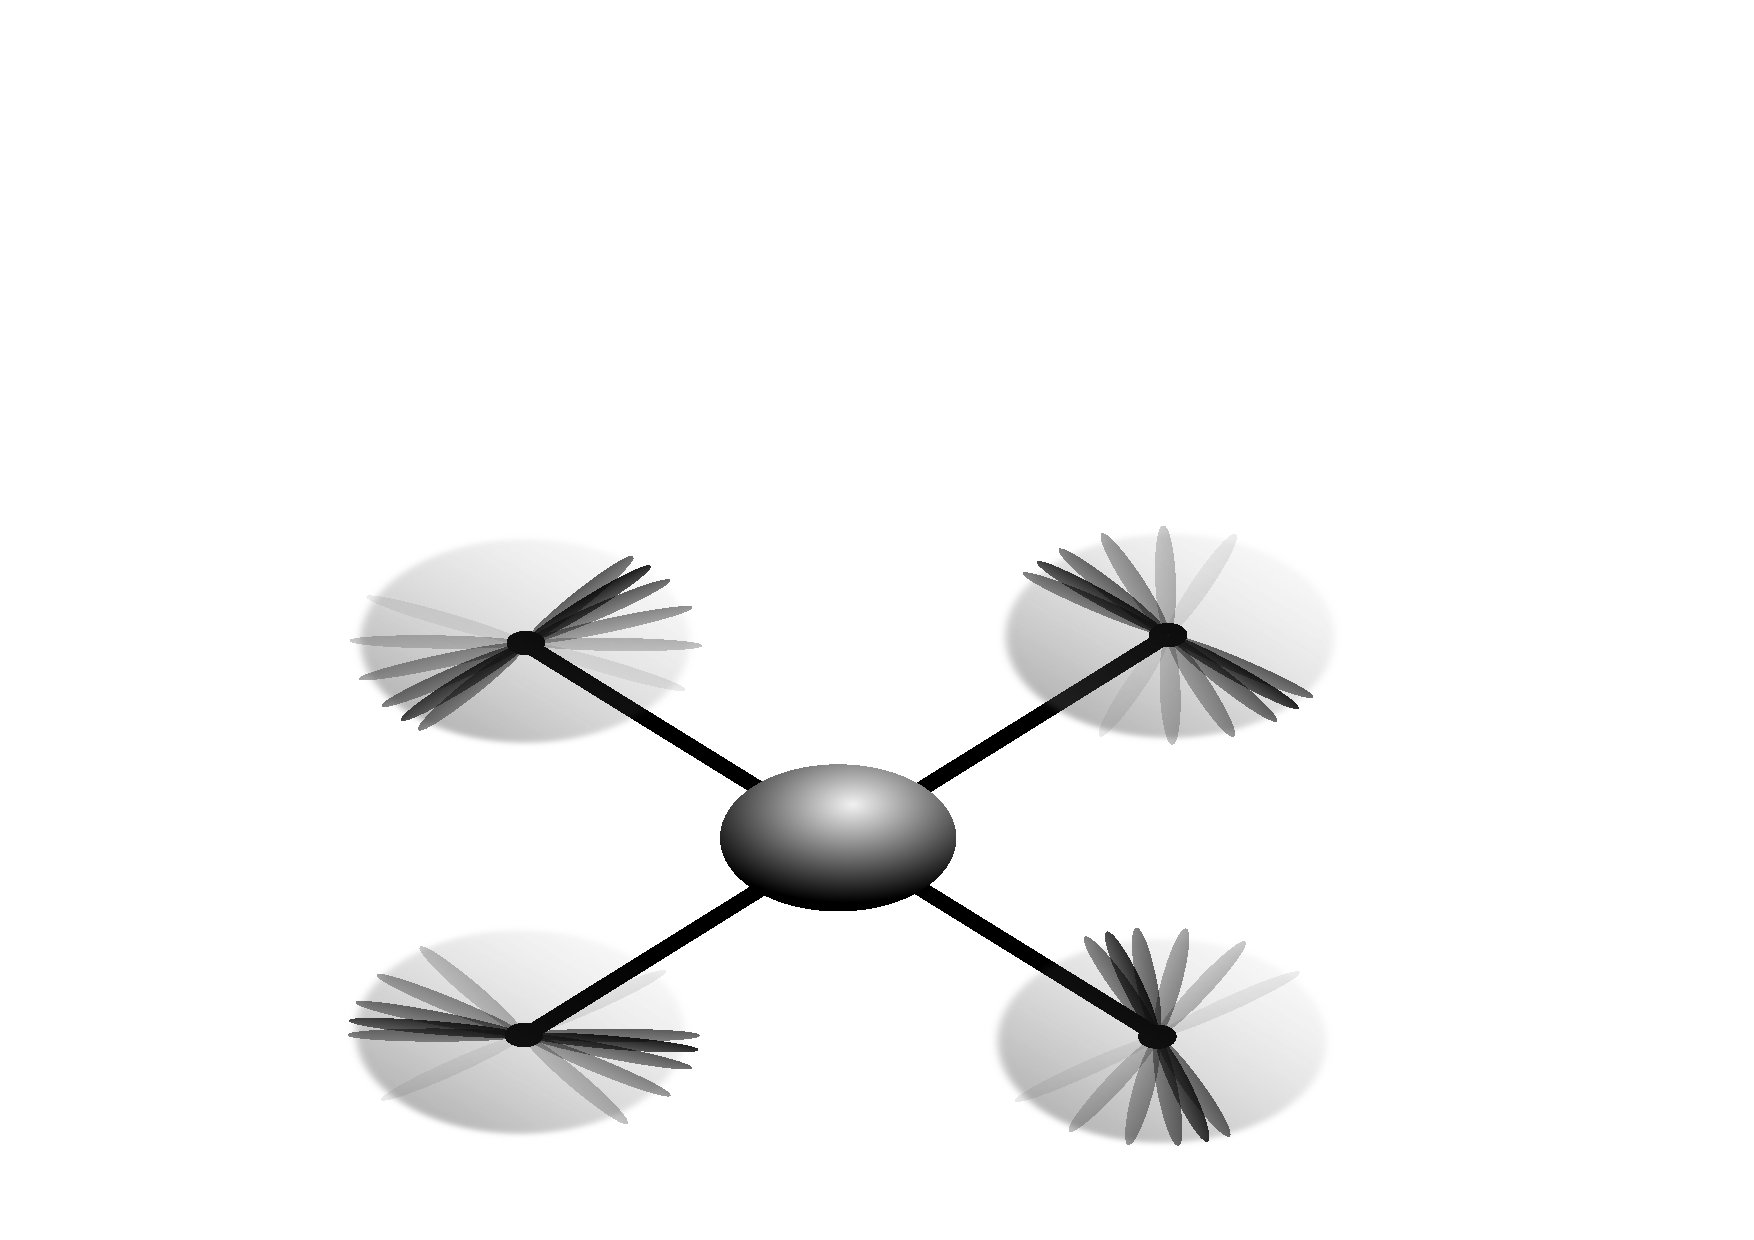
\includegraphics[width=11cm]{images/Copter_leer.pdf}
				\end{figure}
\end{frame}

\begin{frame}
	\frametitle{Forces}
			\begin{figure}[p]
					\centering
					\includegraphics<1>[width=11cm]{images/Copter_Fg.pdf}

					\includegraphics<2>[width=11cm]{images/Copter_Rotorrichtung_zwei.pdf}

					\includegraphics<3>[width=11cm]{images/Copter_Rotorrichtung.pdf}

					\includegraphics<4>[width=11cm]{images/Copter_Rotorkraefte.pdf}
				\end{figure}
\end{frame}

		\begin{frame}
		\frametitle{Forces}
			\begin{columns}[T] % align columns
			\begin{column}{.7\textwidth}
				\begin{textblock}{0}(-2,-6.5)
					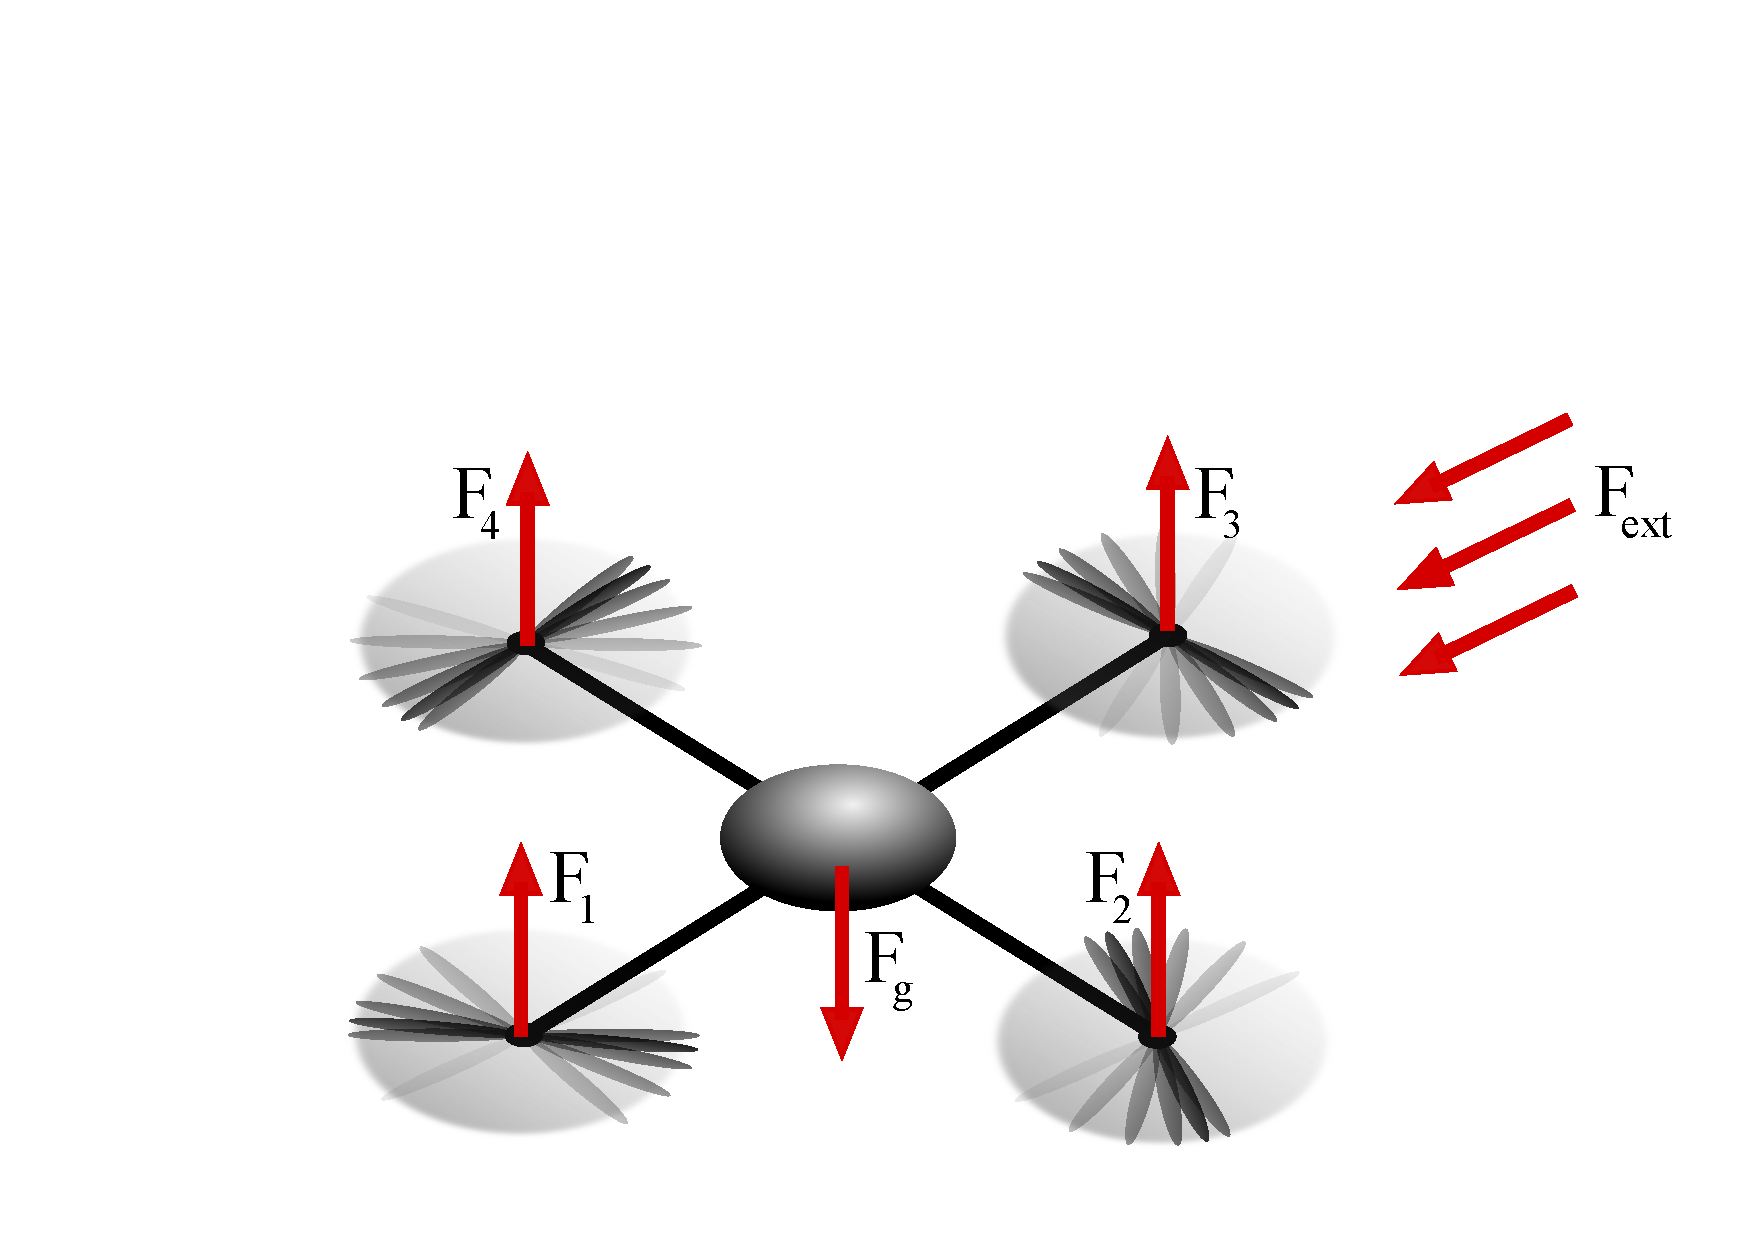
\includegraphics[width=11cm]{images/Copter_Fext_2.pdf}
				\end{textblock}
			\end{column}
			\begin{column}{0.29\textwidth}
				\begin{textblock}{0}(-1,1)
					\[ \mathlarger{F_{ext} = F_{g} + \sum_{i=1}^{4}{F_{i}}} \]
				\end{textblock}
				\end{column}
		\end{columns}
\end{frame}

\begin{frame}
	\frametitle{Torques}
	
			\begin{figure}[p]
					\centering
					\includegraphics<1>[width=11cm]{images/Copter_axis.pdf}
				
					\includegraphics<2>[width=11cm]{images/Copter_phi.pdf}

					\includegraphics<3>[width=11cm]{images/Copter_theta.pdf}

					\includegraphics<4>[width=11cm]{images/Copter_psi.pdf}
				\end{figure}
		
\end{frame}

\begin{frame}
		\frametitle{Torques}
			\begin{columns}[T] % align columns
			\begin{column}{.7\textwidth}
				\begin{textblock}{0}(-1.8,-5.3)
					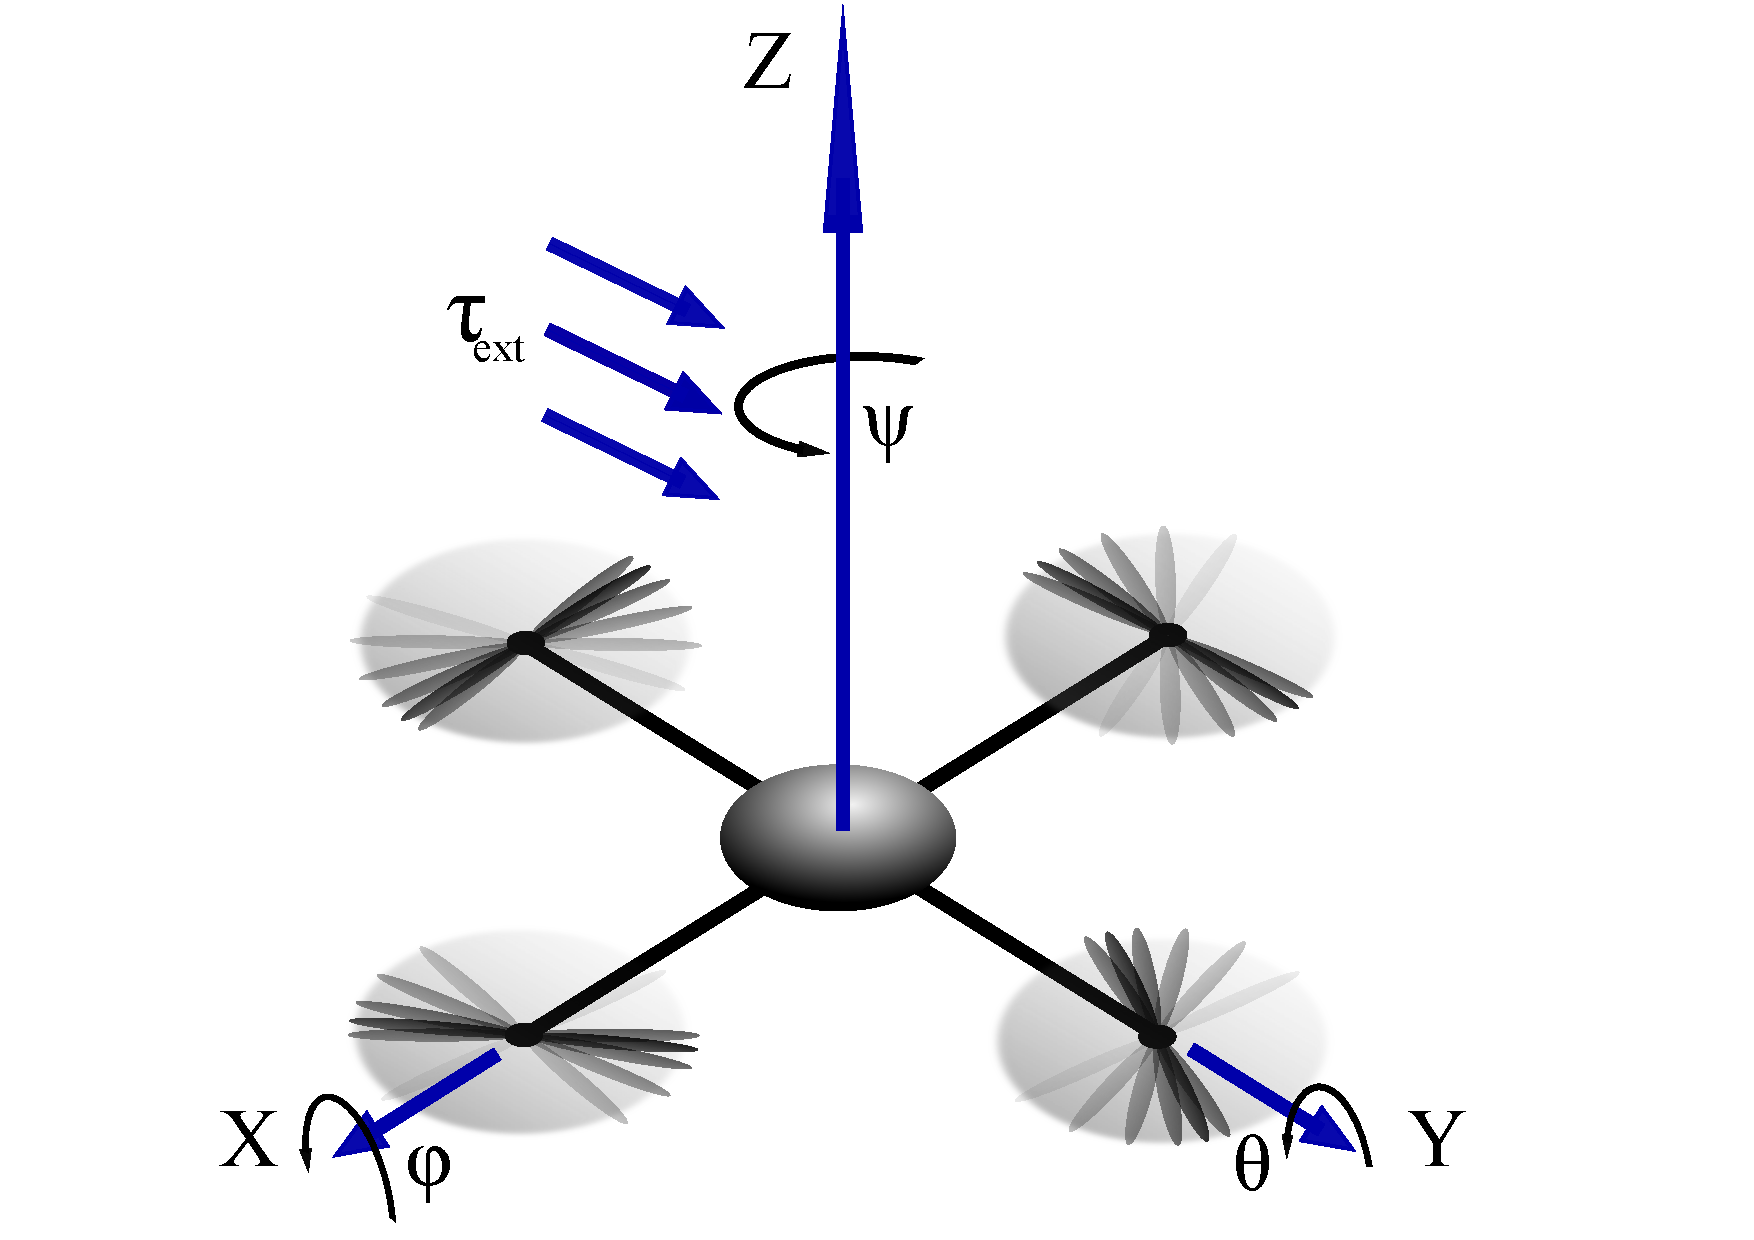
\includegraphics[width=11cm]{images/Copter_Text.pdf}
				\end{textblock}
			\end{column}
			\begin{column}{0.29\textwidth}
				\begin{textblock}{0}(-1.5,1.9)
					\[ \mathlarger{\mathlarger{\tau_{ext} = \tau_{\psi} +\tau_{\varphi}+\tau_{\theta}}} \]
				\end{textblock}
				\end{column}
		\end{columns}
\end{frame}

\begin{frame}
	\frametitle{Obtain ODE}
	\begin{block}{}
		\centering
		\[\left. \begin{array}{c} F_{ext} = F_{g} + \sum_{i=1}^{4}{F_{i}} \\ \tau_{ext} = \tau_{\psi} +\tau_{\varphi}+\tau_{\theta}  \end{array} \right\} \quad \Rightarrow \quad \dot{x}=f(x,u) \]
		\vspace{1ex}
	\end{block}
	
\end{frame}
